\section{Initial Plan}
I am keeping up with project tasks and deadlines in \href{https://linear.app}{linear.app} both for future reference and timestamping the work. Figure \ref{fig:linear} shows how that currently looks and more items will be added as they appear.

\begin{figure}[h]
  \centering
  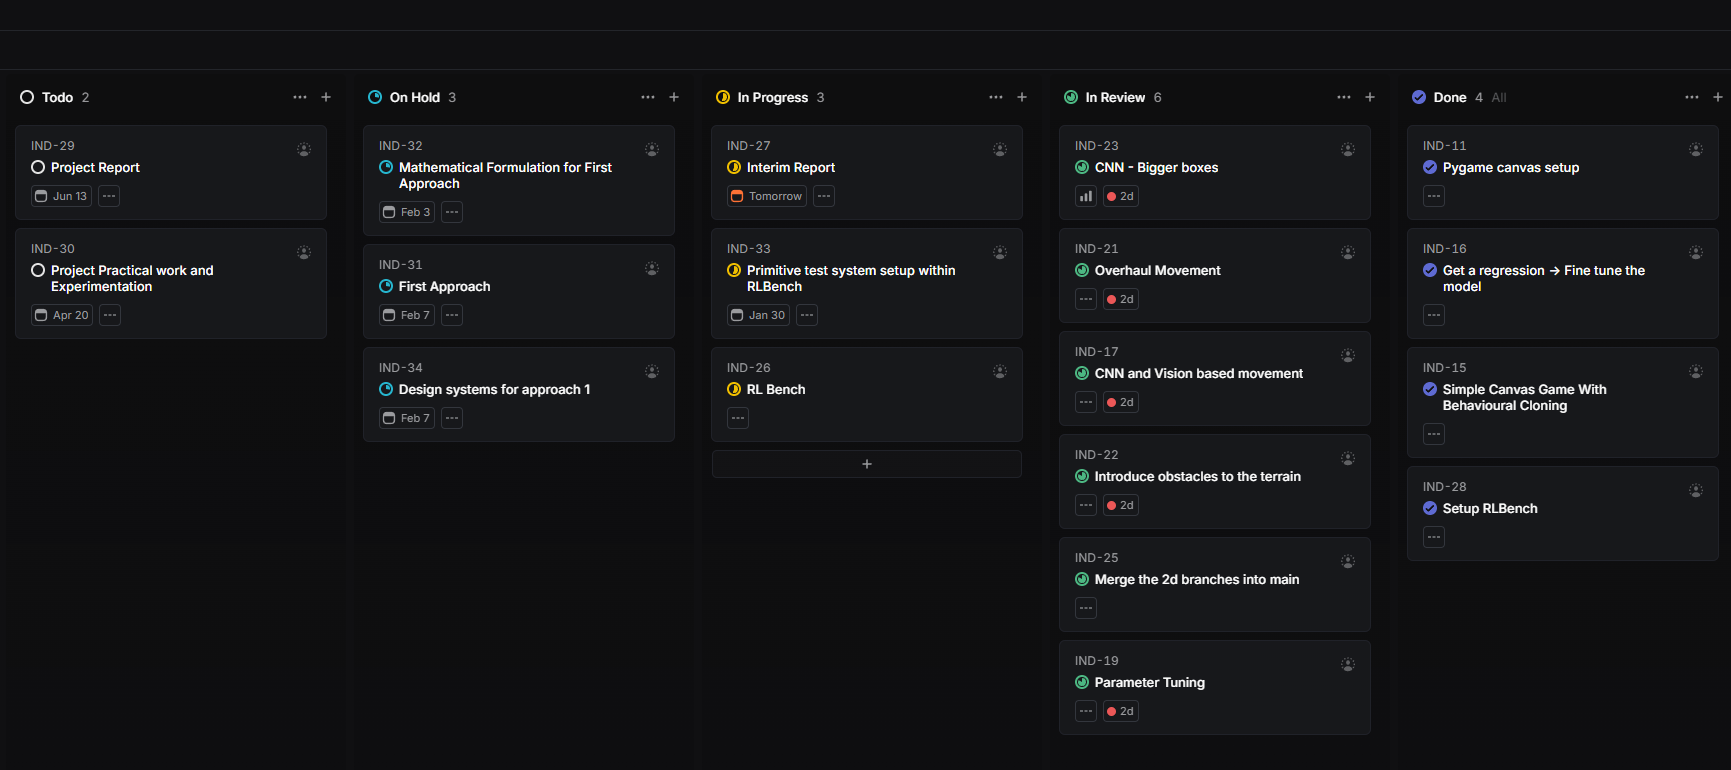
\includegraphics[width=\textwidth]{assets/initial-plan/initial-linear.png}
  \caption{Screenshot of the linear.app interface containing the first week deadlines}
  \label{fig:linear}
\end{figure}



\subsection{Road Map}
I am planning on dividing the project into little segments throughout the the term and the easter holiday. These will be in two week increments fo follow the frequency I meet with my supervisor. There are also some major tasks that are specifically deadlined. Such as, the hard report deadline \DTMdate{2025-06-13} (Top blue box in Figure \ref{fig:ggant}) and the internal deadline I set myself for the project experimentation is \DTMdate{2025-04-20} (second-from-the-top green box from Figure \ref{fig:ggant}). 
The experimentation deadline is designed to have a 10 day biffer and be able to accommodate overflowing to at max \DTMdate{2025-05-01}, so, the final month can be dedicated to making sure the report is comprehensive and complete. I aim to do report work throughout, and expect big updates on the report after experiment results and formulations.

Starting from the deadline of the interim: \DTMdate{2025-01-23}. Here is the outline of the first segment shown in Figure \ref{fig:ggant}.

\begin{figure}[h]
  \centering
  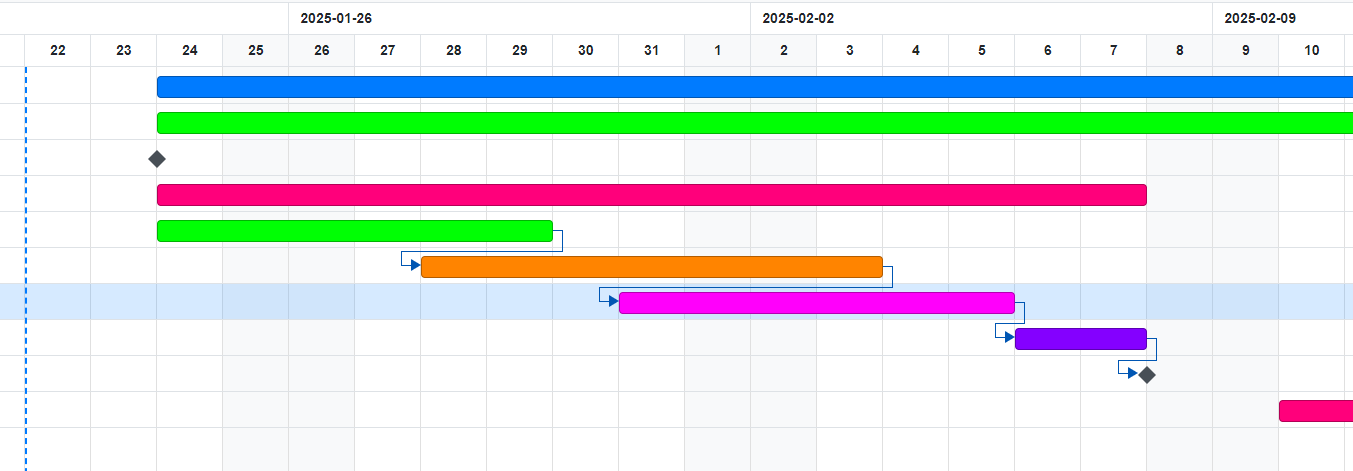
\includegraphics[width=\textwidth]{assets/initial-plan/first-week.png}
  \caption{Ggant Diagram outlining the first week}
  \label{fig:ggant}
\end{figure}

\subsubsection{First Milestone}
Initial plan is to create a rudimentary testing setup within \emph{RLBench} which is the benchmarking framework I started experimenting with (see more \ref{sec:eval-plan}). This is highlighted as the first green box after the first diamond shape in Figure \ref{fig:ggant}

Then, as discussed in the objectives (see \ref{sec:intro-objectives}), I am planning on starting mathematical formulation of the proposed approaches. Formulation will be the orange box. On completing formulation, I will move onto getting a system that attempts ideas from the formulation and possibly use the rudimentary testing system and test this in RLBench or other software as applicable. 

Then, finally, the dark purple box which is for writing out results before presenting to my supervisor on the next day.

\subsubsection{Later Sprints}
I don't expect every sprint to fit perfectly into the 2 weeks allocated. So depending on the size of the task and time it will require, I might allocate two sprints per task, totalling four weeks in total; or maybe half a sprint. Currently, I think this initial task, shouldn't take longer than about 12 days, hence I think a two week period is sufficient.

A quick high-level overview of the deadlines of other tasks are:
\begin{itemize}
  \item Have all approaches (again from \ref{sec:intro-objectives}) formulated and tried out on simulators to some degree by \textbf{\DTMdate{2025-03-15}}
  \item Have a finalised test environment that is robust and can hit criteria conclusively defined later(see \ref{sec:eval-plan}) by \textbf{\DTMdate{2025-04-20} [\DTMdate{2025-05-01} at the latest] }
  \item Have all testing done and report in a ready-to-submit shape by \textbf{\DTMdate{2025-06-01}} (leaving a healthy \~10 day buffer before submission)
\end{itemize}

Other local deadlines will be figured out along the way and will be tracked through linear.app, as mentioned, with minimum buffers of around a week for each, incase the work takes considerably more time than expected.